% !TEX program = xelatex
\input{../../../starter.tex}
\setmainfont[
Ligatures=TeX,
Extension=.otf,
UprightFont= *-regular,
BoldFont=*-bold,
ItalicFont=*-italic,
BoldItalicFont=*-bolditalic]{texgyretermes}



\title{The Effect of Bail on Guilty Pleas\\
\large{\textit{MS\&E 330}}}
\author{
Ali Alkhatib, Nikhil Garg, Martin Lindsey, Danaë Metaxa--Kakavouli
\\
\{\href{mailto:al2@stanford.edu}{al2},
  \href{mailto:nkgarg@stanford.edu}{nkgarg},
  \href{mailto:mlindsey@stanford.edu}{mlindsey},
  \href{mailto:metaxa@stanford.edu}{metaxa}\}@stanford.edu}


\bibliographystyle{apalike}


\begin{document}

\begin{titlingpage}
  \maketitle
\end{titlingpage}

\begin{abstract}
Research on the subject of
bail,
the burden it places on defendants, and
the persuasive and perhaps coercive influence it bears on the justice system
has been explored to some extent ethnographically, but thus far
researchers have not had the data necessary to conduct rigorous quantitative studies on
bail--setting and
the factors which influence pleading behavior. % and the influencing factors therein have not had sufficient data
With a unique insight into the demographics and characteristics of defendants and their outcomes,
we explore two questions:
\begin{inlinelist}
\item Does a greater burden, as measured by bail, cause people to plead guilty? And
\item Are judges handling cases uniquely, or uniformly?
\end{inlinelist}
Our findings reveal that heightened burdens do seem to cause defendants to plead guilty at a higher rate,
and that there is some evidence that variance in bail--setting is unique to judges.
\end{abstract}



\section{Introduction}
%!TEX root = final.tex
Maintaining an efficient justice system is in the interest of both the professionals managing and the citizens interacting with it.
Computational methods including large--scale data analysis and machine learning excel at quantitatively identifying points of inefficiency.
We propose to use these techniques to build models predicting points of inefficiency in the pretrial processes,
in order to provide recommendations for improving efficiency to judges and other court officials.

Notably,
a large majority of cases are never sent to trial; rather,
charges are dropped or settled out of court.
Pretrial procedures,
then,
such as the setting of bail or decision to pursue a case,
are especially fruitful sites for consideration with regards to efficiency.
A more insightful understanding of how to approach these pretrial procedures will benefit court officials in the time and money spent processing cases needlessly.
For defendants,
these insights could lead them to spend less time in prison awaiting trial if they are unable to pay bail,
and fewer resources towards a case that will never be brought to trial.


With this potential for intervention in mind,
we propose to examine the Gotham dataset,
using case features available to the judge,
and in particular bail,
which is set by the judge,
to predict whether a defendant will plead or not later in court proceedings.
The goal of this procedure is to analyze one attribute of a defendant's process through the justice system from the perspective of a judge,
including information the judge knows about the case and,
most importantly,
the decision a judge can make: setting bail.


Specifically,
we conceive of bail setting as imposing a type of (intentional) burden upon a defendant.
This burden can occur at several different levels,
from release on a defendant's own recognizance (ROR) --- a nonexistent burden,
to refusal to set bail at all in order to keep a defendant in custody --- a very high burden.
In between these two levels are bails set which the defendant is able to pay (or find a bondsman to put up bond),
and bails which the defendant is not able to pay.
These two categories are irrespective of the bail amount,
and instead are specific to the means of the defendant who is either able or not to pay bail.
Similarly,
it is worth considering whether different judges set bail in substantially different ways given similar cases,
as a starting point for different analyses.


We make \nextitemizecount{} hypotheses:
\begin{enumerate}
\item Effect of burden on pleading:
      that placing a larger bail burden on a defendant will correlate with a
      higher likelihood to plead later in the case.
      We posit a causal psychological mechanism by which
      defendants who have been required to put up substantial financial assets or,
      even further,
      had to spend time in jail awaiting trial are placed in a vulnerable position
      by the justice system and
      therefore are less likely to prolong their case defend themselves forcefully against charges
      --- in other words, more likely to plead guilty.
\item Our secondary hypothesis predicts that
      different judges will set substantially different bail on similar cases,
      since we anticipate that there is significant room for human error or
      difference this aspect of the justice system.
\end{enumerate}

The underlying goal of this work is
to provide predictions which aid judges in setting effective but
not excessive bail by
better understanding one way in which the process of setting bail influences
defendant experiences with and attitudes toward the justice system.

\section{Literature Review}
%!TEX root = final.tex
Broadly, we identify \nextitemizecount{} areas of research which provide some insight into this topic:
\begin{inlinelist}
  \item The use of
    \textit{\lnameref{subsec:bail}},
    and its stated and empirical purposes,
  \item the study of the effect that bail has on
    \textit{\lnameref{subsec:burden}},
    and
  \item the role of
    \textit{\lnameref{subsec:plea}},
    both for the courts and defendants.
\end{inlinelist}
We will discuss the intersection of these bodies of work as they relate to our research question.


\subsection{\nmu Bail}\label{subsec:bail}
In this section, we will explore the murky waters of the use of bail,
but ultimately settle on the conclusion that the courts have made:
that bail is fundamentally a necessity in a judicial system,
despite the philosophical questions and issues it inherently raises.
Despite the need for bail as a robust safeguard against undue imprisonment,
we will illustrate that the practice of bail--setting is
--- perhaps decidedly --- difficult to discuss in broad terms,
often leaving researchers primarily with
    qualitative,
    ethnographic, and sometimes
    anecdotal
evidence upon which to work.

Bail represents an attempt to resolve a challenging cognitive dissonance.
As \citet{foote1959bail} points out, the imprisonment of a defendant who is nominally considered
``innocent until found guilty''
arouses challenges of principle;
if the courts are to assume that a defendant is innocent (and thus treat them as such),
then holding them in custody until the trial begins is patently wrong, as it deprives a
\textit{presumably} innocent person of freedom.

Nevertheless, the United States Constitution's 8th amendment
--- as well as a series of laws attempting to reform bail
(one in 1966, another in 1984) ---
ostensibly protect defendants from unreasonable and excessive bail amounts,
otherwise to be set at the discretion of the presiding judge
\citep{berg1985bail}.
As \citeauthor{berg1985bail} notes, however,
the most recent revisions to the Bail Reform Act
--- those passed in 1984 ---
make it explicit that judges may set or even deny bail on the basis of
the judge's assessment of the defendant's danger to the community.
In \citet{1984schall},
the court ruled that
``there was nothing inherently unconstitutional in preventive detention''
and that
``the restraint on [the defendant]'s liberty
did not amount to punishment because
that was not the express purpose of the pretrial detention''.

The precedents established in the cases of
\citet{1984schall} and
\citet{1987united} broadly supports the judge's prerogative to set bail
--- and importantly, to \textit{not} set it
(in other words, to remand the defendant with no option to pay bail),
if the judge determines that safety to the community
(or the defendant's appearance upon a later court date)
could not be assured by any bail amount.
This latitude becomes an important component that we attempt to explore
in the hopes of determining whether if
--- at least within a single jurisdiction ---
judge bail--setting variance is high or not.
The implication of this question may be that
some judges are more merciful,
and some decidedly harsher,
than their peers in their assessments of defendants.




\subsection{\nmu Burden}\label{subsec:burden}
The 1984 Bail Reform Act thus
afforded the courts a great deal of freedom in setting bail,
bringing us naturally to the question of what effect this has on defendants awaiting trial.
In this area, we find myriad researchers have contributed;
we will attempt to highlight some of the work that is
especially illuminating and
representative of the body of work.

\citeauthor{kellough2002remand} identify qualitatively that the
``moral assessments'' of defendants appear to influence the burden judges assign in the form of bail--setting.
This, they hypothesize, may explain
(at least to some extent)
the disparity in race between
those that are let free in the interim before their court date, and
those that are held in custody on remand
\citep{kellough2002remand}.

\citeauthor{zacharias1997justice} further discusses the burden that bail may impose on defendants,
in this case highlighting the leverage that prosecutors may have over defendants,
for instance in the form of the unfamiliar and unwelcome environment
that temporary incarceration represents, and the promise to expedite one's interaction with the justice system
\citep{zacharias1997justice}.
This, finally, leads us to the outcome variable which we will ultimately investigate.


\subsection{\nmu Plea \nmu Bargaining}\label{subsec:plea}
Most tangibly, the persuasive
(perhaps \textit{coercive})
force that prosecutors can exercise in tandem with judges is
the pressure to encourage defendants to plead guilty in the pretrial phase.
This aspect of the justice system is especially unique, both because
plea--bargaining defies the adversarial model of the court and trial process and because
these dynamics are so ill--understood at broad levels
\citep{zacharias1997justice}.

The research on the \lnameref{subsec:burden} that bail represents on defendants
--- especially defendants with limited financial means and similarly limited access to cash ---
has \textit{qualitatively} found that
trial outcomes may be affected by the burden of pretrial incarceration.
To illustrate this, we turn to
\citet{grossman1983plea} and \citet{alschuler1981changing};
\citeauthor{grossman1983plea} estimates that as many as
``90 percent of convictions \dots result from a negotiated plea of guilty''
\citep[see also][with similar findings]{mccoy1980plea,kaplan1977american,newman1966conviction}.

Most of the existing research in plea bargaining,
especially \citeauthor{grossman1983plea}'s work,
focuses on the economic role of the plea bargain as a
``screening device'';
\citeauthor{alschuler1981changing}
contributes to the argument that pretrial bargaining may serve the defendant's best interests,
observing that neither the courts nor the public defenders who often represent defendants
have sufficient time to see all cases through open court
\citep{alschuler1981changing}.
\citeauthor{alschuler1981changing}
makes the noteworthy observation that we lack sufficient information to determine whether 
  the pressure of incarceration,
  the prosecutor's persuasive offer to settle, and
  the defending attorney's desire to expedite the closure of outstanding cases
is in fact causing defendants to settle more frequently,
primarily due to a dearth of broad--based data, and certainly
--- as \citeauthor{kellough2002remand} describe it ---
a simple ``paucity of research [in plea bargaining]''
\citep{kellough2002remand}.





\section{Method}
%!TEX root = final.tex
In order to analyze our two research questions,
we first quantify bail burden and preprocess the data,
and subsequently perform statistical analyses on the data.
The methods used in these steps are detailed below.


\subsection{Bail Burden}
We conceive of the possible burden placed on a defendant by bail as fitting into one of
\nextitemizecount{} categories:
\begin{inlinelist}
  \item When a defendant is Released on his or her Own Recognizance (ROR),
  the burden is negligible.
  Defendants are required neither to put up money nor to spend time incarcerated; 
  \item when bail is set and a defendant is able to pay it immediately,
  the defendant is lightly burdened; 
  \item when bail is set and a defendant is able to pay it but with a delay,
    the defendant is significantly burdened both
    financially and by
    needing to spend time incarcerated prior to meeting bail; 
  \item when a defendant either has no option to be released on bail,
  or is unable to meet bail,
    he or she is \textit{severely} burdened,
    having to spend the entire time until trial incarcerated.
\end{inlinelist}

\subsection{Preprocessing}
Several preprocessing steps were taken to ensure the validity of our analyses.
Due to some inconsistencies in volume of cases prior to 2013,
only cases from after (and including) 2013 were analyzed.
Additionally,
cases involving violent offenses were removed since
there are extra considerations and complexities in bail--setting for violent offenders,
who may be considered safety risks to the community and evaluated differently for bail.
We also only consider cases that made it past arraignment,
since cases where charges were dropped at arraignment are ineligible for the analyses we perform.
Finally,
for most analyses we consider Quality of Life (QoL) and non--Quality of Life (non--QoL) offenses separately.
Quality of life offenses make up a category of illegal activity which is connected with the broken windows theory of policing
--- these are misdemeanor offenses such as
  disorderly conduct,
  vagrancy,
  or
  loitering.
QoL and non--QoL offenses may differ substantially in the populations being charged and in their handling in the justice system,
so we perform the same analyses in parallel across these two types of data.



\subsection{Analyzing the Effect of Bail on the Probability to Plea}
We analyze the effect of bail burden on the probability of pleading through
two main techniques and
using both random forest models and GLM.
First,
we train models to predict the probability of pleading using all case characteristics through arraignment,
including the burden level set.
Then we create test sets composed of different burden levels
(through two different techniques,
described next),
and analyze the test set probability of pleading conditional on each burden level.
We present the results both as a CDF of the test sets' probability of pleading and as means of the distribution.

To verify the effectiveness of our models,
we produce calibration plots and include them in the appendix.
For each row in the original test set,
we predict the probability of pleading and ROR,
respectively,
for our two models.
We bin these probabilities and observe the true probability of observing the dependent variable for each of the bins.


\subsubsection{``All Else Equal''}
For our preliminary analysis,
we create the test sets for each burden level through an ``all else equal'' assumption
--- that we can change the burden level of a given case while holding all other case characteristics the same.
We duplicate the test set into four sets.
In each data set,
we set the burden level to
  ``ROR'',
  ``Trivial'',
  ``Trivial with Delay'',
  and
  ``Jail'',
respectively.
We then send these test sets to the model and view the resulting predicted probability of pleading.
We note that the ``all else equal'' assumption is not true in general.
In a murder case,
for example,
it would not make sense to change the burden level from ``Jail'' to ``ROR''.
However,
because we analyze only non--violent cases,
the assumption holds approximately.



\subsubsection{Propensity Score Matching}
To further support our analysis,
we relax the assumption through initial propensity score matching.
For this method,
we split the burden into only two levels: ROR and Non--ROR.
We train a model to predict the probability of ROR.
Two test sets are then matched on the probability of ROR through \texttt{matchit}
\citep{matchit},
and the burden bits are set to ROR and Non--ROR,
respectively.
They are then sent to the probability of pleading models.
To do true propensity score matching and make sure our assumption holds,
we should have filtered out cases with either very low or very high probability of ROR.
Otherwise,
we are still using cases where it would not make sense to change the ROR value.


\subsection{Analyzing the Effect of Judge on Bail}
\subsubsection{Analysis --- Random Forest}
For an initial analysis to observe judge effects,
we predict the Probability of ROR being granted for each case,
without using \texttt{JudgeID} in our prediction model.
This analysis uses the same Random Forest ROR model trained in the Propensity Matching analysis.
This model gives a baseline for judge independent granting of ROR.
For each judge with over 100 cases in the test set,
we determine the judge's mean predicted probability of ROR using the model.
This value is the percentage of a given judge's cases that the ``average'' judge would ROR.
We compare this value to the true percentage of cases in which each judge actually granted ROR.

\subsubsection{Analysis --- Generalized Linear Model}
An ``all else equal'' approach was taken in the GLM analysis
--- the general strategy was to create a copy of the data with a test variable set to a given value,
input these modified datasets into the model for each value the test variable can assume,
and then obtain summary statistics for each possible value
to then compare with the summary statistics associated with the other values;
by doing this,
any predictive power this model might have can be used
to check for the relative influences of certain factors on the outcome that this model predicts.

The ROR model was used to check if certain arraignment judges differed substantially in how they treated ROR.
The plea model was used to check if certain levels of burden had a higher predicted rate reaching a plea disposition.
As a cursory additional check,
matching edge cases were identified using a software package
(i.e. cases that can be considered similar on model inputs but differed on observed outcomes),
and in each case,
the same analysis was performed on a reduced dataset of these edge cases to similar results.

Within this reduced set of edge cases,
the assumption of ``all else equal'' has greater validity,
as the matching software is trusted to compute a quantitative measure of this
``equality'' between cases and identify precisely those which are ``sufficiently equal''.
The effects of judge on ROR are summarized in
figures~\ref{fig:ROR_QoL_GLM} and
        \ref{fig:ROR_non--QoL_GLM}.
For non--QoL cases,
judges seem to have more similar ROR rates compared to QoL cases
(one of the most prolific judges is also an outlier in the QoL dataset).
The effects of burden on the rate of plea dispositions are summarized in
figures~\ref{fig:QoL_plead_GLM} and
        \ref{fig:non--QoL_plead_GLM}.

For both QoL and non--QoL cases,
the lower levels of burden had close distributions,
but the distribution for ``nontrivial'',
the highest level of burden had its mass shifted noticeably toward higher plea rates.
Additionally,
the predicted plea distributions on the QoL dataset had mass shifted more to the right compared to the non--QoL distributions.
Analogous plots for the same analysis performed with the ROR model on the matched non--QoL dataset are found in
figures~\ref{fig:mean_ROR_non--QoL_GLM} and
        \ref{fig:mean_ROR_QoL_GLM};
the other combinations of QoL or non--QoL and ROR or plea model yielded matched datasets that were too small
(i.e. on the order of tens of cases) to use.









\section{Results}
%!TEX root = final.tex
\subsection{Analyzing the Effect of Bail on the Probability to Plea}
\subsubsection{All Else Equal --- Random Forest}
We first carry out the All Else Equal analysis through a Random Forest model.
Appendix \ref{appendixA} shows the calibration information for the Random Forest models for both
Non--Quality of Life and
Quality of Life cases.
We observe that the models are accurate and serviceable,
though the Non--QoL model consistently over--predicts the probability of pleading in the unaltered test set.

Tables~\ref{table:non--QoL_plead} and
       \ref{table:QoL_plead},
respectively,
include the mean predicted probability of pleading at different burden levels for
Non--Quality of Life and
Quality of Life cases, respectively.
Figures~\ref{fig:non--QoL_plead} and
        \ref{fig:QoL_plead}, show the CDFs of same values determined through the model.
Applying the GLM to the dataset reveals roughly similar predictions, as illustrated by
Figures~\ref{fig:non--QoL_plead_GLM} and
        \ref{fig:QoL_plead_GLM}.


We observe that,
especially for Non--Quality of Life cases,
jailing someone substantively increases the predicted probability of pleading when compared other burden levels.
This effect can be observed through both the higher means and the right--shift on the CDF plots.
The effect is similar, though much less pronounced, for Quality of Life cases.

\begin{table}
\centering
\begin{tabular}{|p{0.3\textwidth}|p{0.6\textwidth}|}
  \hline
\textbf{Burden Level} & \textbf{Mean Predicted Probability of Pleading} \\ \hline
    ROR & 0.3631537 \\ \hline
    Trivial & 0.3834242 \\ \hline
    Delay & 0.3744825 \\ \hline
    Jail & 698843  \\ \hline
  \end{tabular}
  \caption{Mean Probability of Pleading for Non--Quality of Life offenses through All Else Equal Analysis using Random Forest model}
  \label{table:non--QoL_plead}
\end{table}

\begin{table}
\centering
\begin{tabular}{|p{0.3\textwidth}|p{0.6\textwidth}|}
  \hline
\textbf{Burden Level} & \textbf{Mean Predicted Probability of Pleading} \\ \hline
    ROR & 0.6072936 \\ \hline
    Trivial & 0.6102411 \\ \hline
    Delay & 0.5999771 \\ \hline
    Jail & 0.648984 \\ \hline
  \end{tabular}
  \caption{Mean Probability of Pleading for Quality of Life offenses through All Else Equal Analysis using Random Forest model}
  \label{table:QoL_plead}
\end{table}


\begin{figure}[t!]
  \centering
  \begin{subfigure}[b]{0.49\textwidth}
    \caption{Non--Quality of Life cases}
    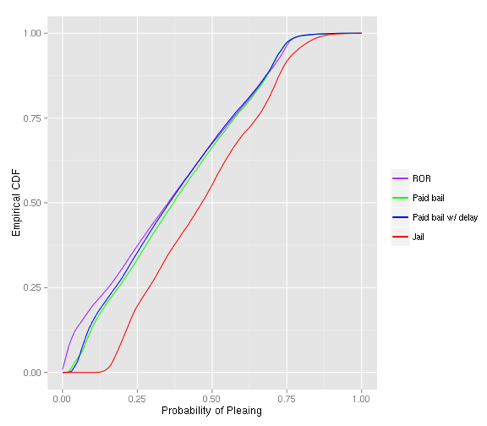
\includegraphics[width=\textwidth]{figures/figx.png}
    \label{fig:non--QoL_plead}
  \end{subfigure}
  ~
  \begin{subfigure}[b]{0.49\textwidth}
    \caption{Quality of Life cases}
    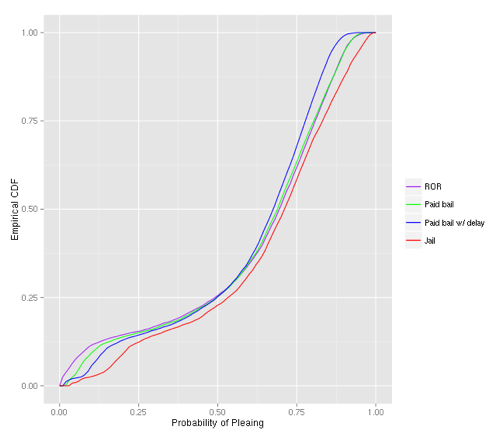
\includegraphics[width=\textwidth]{figures/figy.png}
    \label{fig:QoL_plead}
  \end{subfigure}
  \caption{CDFs of predicted probability of pleading guilty at different burden levels
           determined through the All Else Equal Random Forest model}
  \begin{subfigure}[b]{0.49\textwidth}
    \caption{Non--Quality of Life cases}
    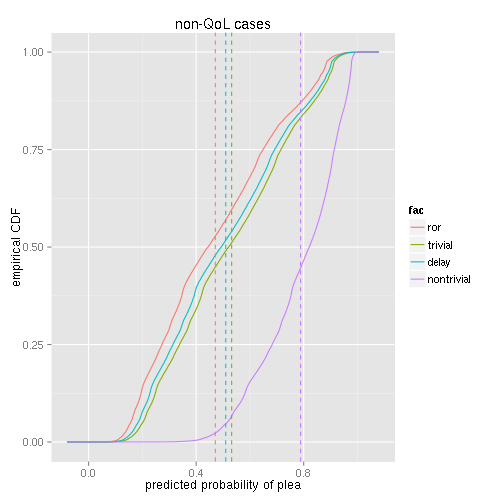
\includegraphics[width=\textwidth]{figures/glmplots/plea_cdf.png}
    \label{fig:non--QoL_plead_GLM}
  \end{subfigure}
  ~
  \begin{subfigure}[b]{0.49\textwidth}
    \caption{Quality of Life cases}
    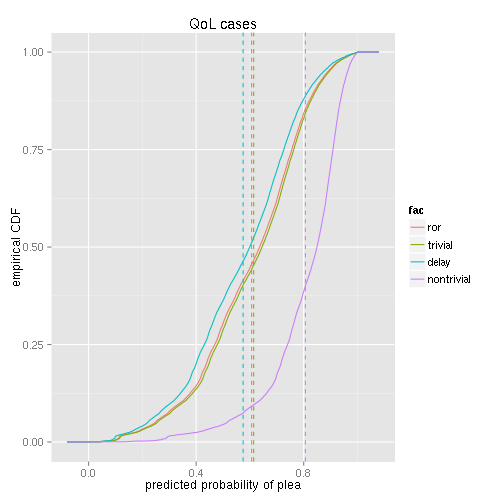
\includegraphics[width=\textwidth]{figures/glmplots/pleaq_cdf.png}
    \label{fig:QoL_plead_GLM}
  \end{subfigure}
  \caption{CDFs of predicted probability of pleading guilty at different burden levels
           determined through the Generalized Linear Model}
\end{figure}


\subsubsection{Propensity Score Matching --- Random Forest}
Finally, we carry out the Propensity Score analysis through a Random Forest model.
Appendix \ref{appendixA}
also includes the calibration information for the Random Forest models to predict ROR for each type of case.
We observe that the ROR prediction models are accurate and unbiased.

Tables \ref{table:ROR_non--QoL_propensity_score} and
       \ref{table:ROR_QoL_propensity_score},
respectively, include the mean predicted probability of pleading for
  ROR and Non--ROR, for
  Non--Quality of Life and Quality of Life cases,
  respectively.
Figures~\ref{fig:ROR_non--QoL_propensity_score} and
        \ref{fig:ROR_QoL_propensity_score} show
the CDFs of same values determined through the model
(also see findings through GLM approach in
Figures~\ref{fig:ROR_non--QoL_GLM} and
        \ref{fig:ROR_QoL_GLM}).


Our results match the All Else Equal analysis.
Especially for Non--Quality of Life cases, a Non--ROR burden level increases the predicted probability of pleading.
Future work should repeat this analysis using
Jail and
Non--Jail burden levels,
as those levels are where the substantive difference occurs in the All Else Equal analysis.


\begin{table}
\centering
  \begin{tabular}{|p{0.3\textwidth}|p{0.6\textwidth}|}
    \hline
    \textbf{Burden Level} & \textbf{Mean Predicted Probability of Pleading} \\ \hline
    ROR & 0.3706164 \\ \hline
    Non--ROR & 0.412566 \\ \hline
  \end{tabular}
  \caption{Mean Probability of Pleading for Non--Quality of Life offenses through Random Forest Modeling}% Propensity Score Matching}
  \label{table:ROR_non--QoL_propensity_score}
\end{table}


\begin{table}
\centering
  \begin{tabular}{|p{0.3\textwidth}|p{0.6\textwidth}|}
    \hline
    \textbf{Burden Level} & \textbf{Mean Predicted Probability of Pleading} \\ \hline
    ROR & 0.6127946 \\ \hline
    Non--ROR & 0.6363191 \\ \hline
  \end{tabular}
  \caption{Mean Probability of Pleading for Quality of Life offenses through Random Forest Modeling}% Propensity Score Matching}
  \label{table:ROR_QoL_propensity_score}
\end{table}


\begin{figure}
  \centering
  \begin{subfigure}[b]{0.49\textwidth}
    \caption{Non--Quality of Life cases}
    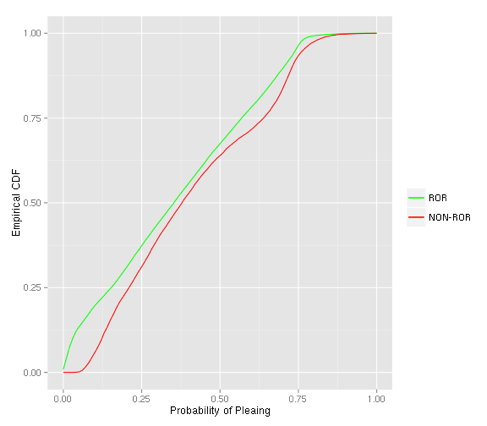
\includegraphics[width=\textwidth]{figures/figxx.png}
    \label{fig:ROR_non--QoL_propensity_score}
  \end{subfigure}
  ~
  \begin{subfigure}[b]{0.49\textwidth}
    \caption{Quality of Life cases}
    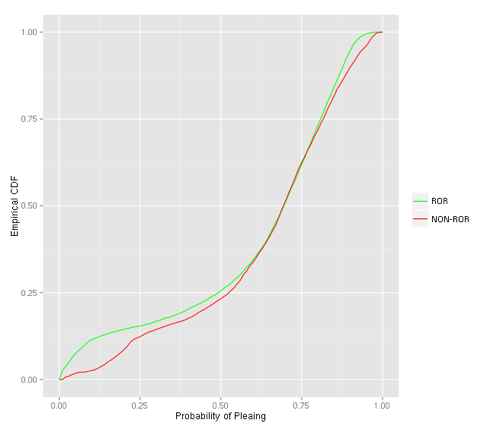
\includegraphics[width=\textwidth]{figures/figyy.png}
    \label{fig:ROR_QoL_propensity_score}
  \end{subfigure}
  \caption{CDFs for the mean predicted probability of pleading for ROR and non--ROR through Random Forest Modeling}% Propensity Score Matching}
  \begin{subfigure}[b]{0.49\textwidth}
    \caption{Non--Quality of Life cases}
    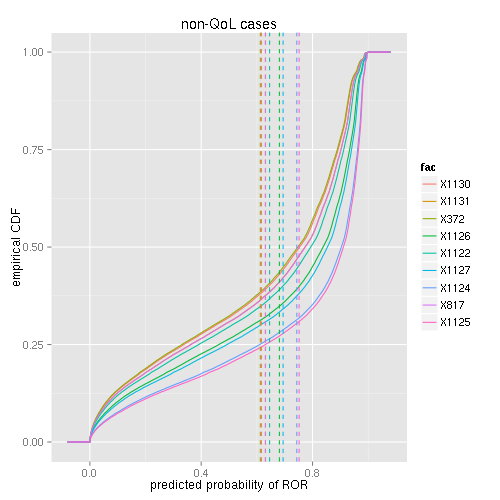
\includegraphics[width=\textwidth]{figures/glmplots/ror_cdf.png}
    \label{fig:ROR_non--QoL_GLM}
  \end{subfigure}
  ~
  \begin{subfigure}[b]{0.49\textwidth}
    \caption{Quality of Life cases}
    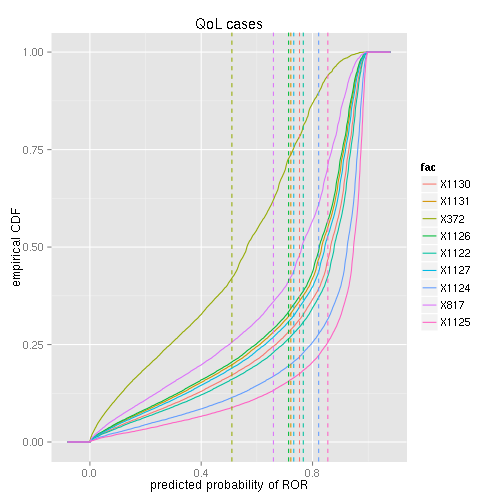
\includegraphics[width=\textwidth]{figures/glmplots/rorq_cdf.png}
    \label{fig:ROR_QoL_GLM}
  \end{subfigure}
  \caption{CDFs for the mean predicted probability of pleading for ROR and non--ROR through Generalized Linear Model}
\end{figure}


\begin{figure}
  \centering
  \begin{subfigure}{0.49\textwidth}
    \caption{Non--Quality of Life cases}
    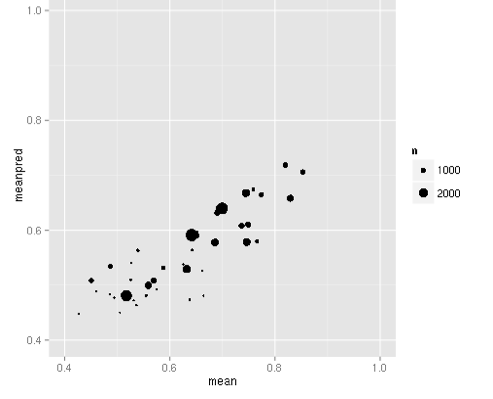
\includegraphics[width=\textwidth]{figures/figaa.png}
    \label{fig:mean_ROR_non--QoL}
  \end{subfigure}
  ~
  \begin{subfigure}{0.49\textwidth}
    \caption{Quality of Life cases}
    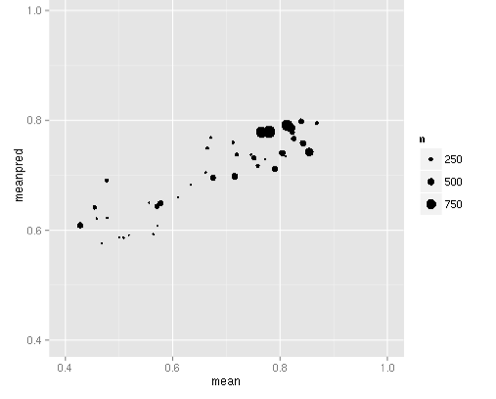
\includegraphics[width=\textwidth]{figures/figbb.png}
    \label{fig:mean_ROR_QoL}
  \end{subfigure}
  \caption{mean probability of ROR for each judge, vs.
  actual percentage of ROR modeled by Random Forest}

  \begin{subfigure}{0.49\textwidth}
    \caption{Non--Quality of Life cases}
    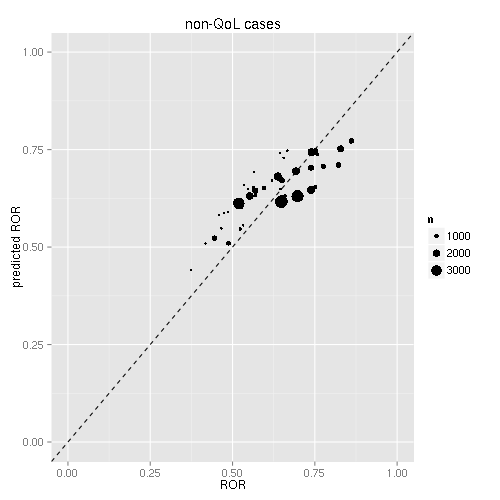
\includegraphics[width=\textwidth]{figures/glmplots/ror_scatter.png}
    \label{fig:mean_ROR_non--QoL_GLM}
  \end{subfigure}
  ~
  \begin{subfigure}{0.49\textwidth}
    \caption{Quality of Life cases}
    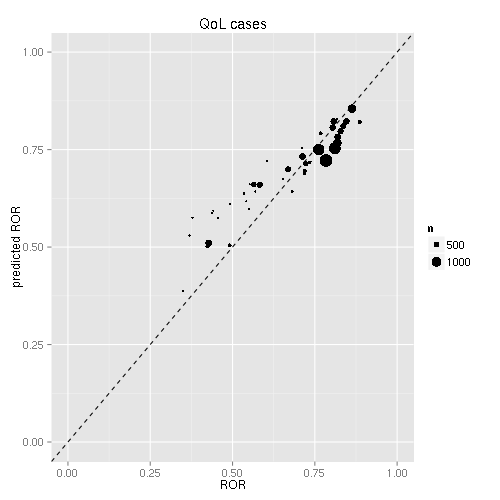
\includegraphics[width=\textwidth]{figures/glmplots/rorq_scatter.png}
    \label{fig:mean_ROR_QoL_GLM}
  \end{subfigure}
  \caption{mean probability of ROR for each judge, vs.
  actual percentage of ROR modeled by GLM}
\end{figure}


\subsection{Analyzing the Effect of Judge on Bail}
Figures~\ref{fig:mean_ROR_non--QoL} and
        \ref{fig:mean_ROR_QoL} show
        the mean predicted probability of ROR
        for each judge versus the judge's actual percentage of ROR,
        for Non--Quality of Life and Quality of Life cases,
respectively.
The plots show that some of the variation in
the judges' percentage of cases that are granted ROR is due to
non--randomness in the cases that they adjudicate.
However,
we observe that for a given mean predicted probability of ROR (on the Y axis),
there is significant judge variance on the true percentage of cases that are granted ROR.
Thus,
this initial analysis shows that different judges do utilize ROR differently for the same types of cases.
As before,
figures~\ref{fig:mean_ROR_non--QoL_GLM} and
        \ref{fig:mean_ROR_QoL_GLM} illustrate similar patterns using a different modeling approach (GLM).

\section{Discussion}
\documentclass[trackingWork]{subfiles}
\makeatletter
\def\blx@maxline{77}
\makeatother
\begin{document}
\section{Discussion}
\topic{Having taken a comprehensive look toward crowd work through the piecework lens,
we can't help but take a step back to consider a number of meta--issues that arose in our analysis.}
Stated briefly, these issues are 
\begin{inlinelist}
  \item \namerefl{sec:perilousProblemsPredicting},
  \item \namerefl{sec:polarizationOfCrowdWork}, and
  \item \namerefl{sec:whatShouldBeTheFuture}.
\end{inlinelist}
We will attempt to grapple with these questions here based on
what we brought up in the earlier case studies.


\subsection{The Hazards of Predicting the Future}\label{sec:perilousProblemsPredicting}
\begin{enumerate}
  \item The past isn't a perfect indicator of the future
  \item ``it would be wrong to conclude that
        in the realm of digital labor
        there is nothing new under the sun''
        \cite{scholz2012digital}.
  \item Digital sites of labor are so radically different
        (for many of the reasons that \DO
        articulated in the discussion about
        organizing people and the challenges therein
        \cite{dynamo}, as well as for
        many of the rhizomatic features \citeauthor{miller2011understanding}
        discusses
        \cite{miller2011understanding}).
\end{enumerate}


\subsection{Polarizing Tendencies}\label{sec:polarizationOfCrowdWork}
\begin{enumerate}
  \item It's easy to think crowd work as heading toward some extreme
  \item Activists describe speculative workers as having
        ``essentially been turned into modern--day slaves''
        \cite{activistsHuffPoLawsuit}.
  \item Meanwhile, advocates describe it as
        ``a project of sharing
        aimed at providing ordinary people
        with more economic opportunities and
        improving their lives\dots''
        \cite{uberPropaganda}.
  \item There may be truth buried in both claims, but the important takeaway is that
        the closest we can get to a single truth is somewhere in the middled,
        buried in nuance.
  \item There may be a Utopian world at the end of the tunnel that is our world now:
        all work that we engage in could become speculative and risky;
        the layers between us and our managers might increasingly become
        ``defective (simple, observable)'' algorithms \cite{10.2307/2555446}
        --- the same ones which already seem to frustrate
        on--demand workers on Uber and other markets for labor
        \cite{uberAlgorithm,dynamo,turkopticon}.
  \item On the other hand, the future of crowd work could be eminently promising:
        piecework's nascent years were nothing short of grim, but
        they precipitated a century of the strongest labor advocacy the world has ever seen.
        In India, workers across the nation engaged in
        the largest labor strike in human history
        % \cite{indiaStrikeIndustriall,indiaStrikeAlJazeera}
        --- perhaps as many as 150 million
        \cite{indiaStrikeRealNews}.
        Arguably the Internet has made collective action on an unprecedented scale much easier.
  \item So are we heading toward \textit{Mad Max} or\dots
        \ali{is there a Utopian future movie?}
        If we do nothing, probably somewhere in the middle.
        It's possible that the difficulties of enforcing laws on multinational corporations is
        tipping the balance of power in the direction of corporations, in which case
        things will get worse;
        but arguably we can affect change on the trajectory of crowd work,
        benefiting from everything piecework scholars have learned about
        collective action and governance
        among workers, while also avoiding some of the perils they faced.
\end{enumerate}

\subsection{Deciding our Research Agenda}\label{sec:whatShouldBeTheFuture}
\begin{enumerate}
  \item We need to take a step back from the work that's been done so far and
        think about where we are going with the crowd work research agenda.
  \item Piecework researchers pointed out long ago that piecework is problematized by the fact that
        ``piecework does not compensate workers for time spent switching tasks''
        \cite{bewley1999wages} --- we've studied this phenomenon in crowd work
        \cite{delayAndOrderLasecki,taskSearch}
        and we should consider whether this remains a worthwhile area to explore unless
        we're actually finding ways to minimize the many forms of costs of switching tasks.
  \item What questions are we trying to answer?
        If, as we assumed in
        the previous section on \namerefl{sec:polarizationOfCrowdWork},
        our driving motivation is to empower workers, we 

\end{enumerate}

\endnotetext{
\begin{enumerate}
  \item the past is no guarantee of the future; what could be unforeseen?
  \item it's easy to fall into the (dys|u)--topian camp of what piecework/crowd work will look like
  \item what should we be focusing on? the future of crowd work
\end{enumerate}
}


\onlyinsubfile{
  \balance{}
  \printbibliography
}

\end{document}

\section{Conclusion}
\documentclass[trackingWork]{subfiles}
\makeatletter
\def\blx@maxline{77}
\makeatother

\onlyinsubfile{
\usepackage{xr-hyper}
\usepackage{hyperref}
\externaldocument{complexity}
\externaldocument{decomposition}
\externaldocument{relationships}
}

\begin{document}
\section{Conclusion}
On--demand work is not new, but a contemporary instantiations of piecework.
In this paper, we reconsider three major research questions in on--demand work using the lens of piecework:
\begin{inlinelist}
  \item \nameref{sec:complexity}?
  \item \nameref{sec:decomposition}?
  \item \nameref{sec:relationships}?
\end{inlinelist}
To do so, we draw on piecework scholarship to inform analyses of what has changed, what hasn't, and may change change soon.
Reciprocally, we believe that modern on--demand work will teach us about the broader phenomenon of piecework as well.
If history really does repeat itself, the best we can do is be prepared.

\end{document}

%!TEX root = final.tex
\newpage
\appendix
\section{Appendix} \label{appendixA}
Below we provide further details including confusion matrices and
reliability plots on some of the models used.

\begin{figure}[h]
  \centering
    \begin{subfigure}[p!]{\textwidth}
            \caption{Non--Quality of Life Cases}
            \begin{subfigure}[p!]{0.49\textwidth}
              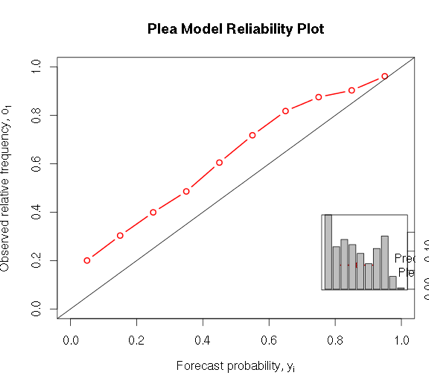
\includegraphics[width=\textwidth]{figures/appa.png}
              \label{fig:AppA}
            \end{subfigure}
            ~
            \begin{subfigure}[p!]{0.49\textwidth}
              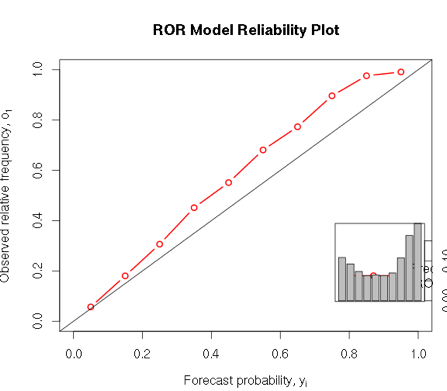
\includegraphics[width=\textwidth]{figures/appb.png}
              \label{fig:AppB}
            \end{subfigure}
    \end{subfigure}

    \begin{subfigure}[p!]{\textwidth}
                \caption{Quality of Life Cases}
                \begin{subfigure}[p!]{0.49\textwidth}

                  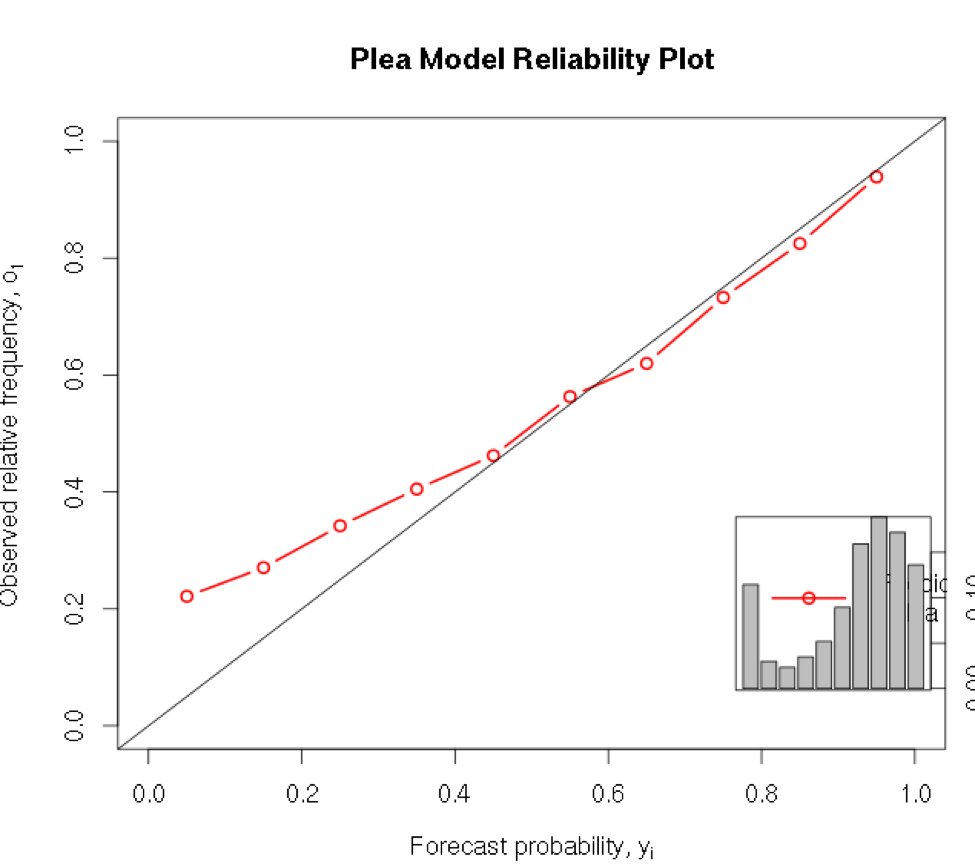
\includegraphics[width=\textwidth]{figures/appc.png}
                  \label{fig:AppC}
                \end{subfigure}
                ~
                \begin{subfigure}[p!]{0.49\textwidth}

                  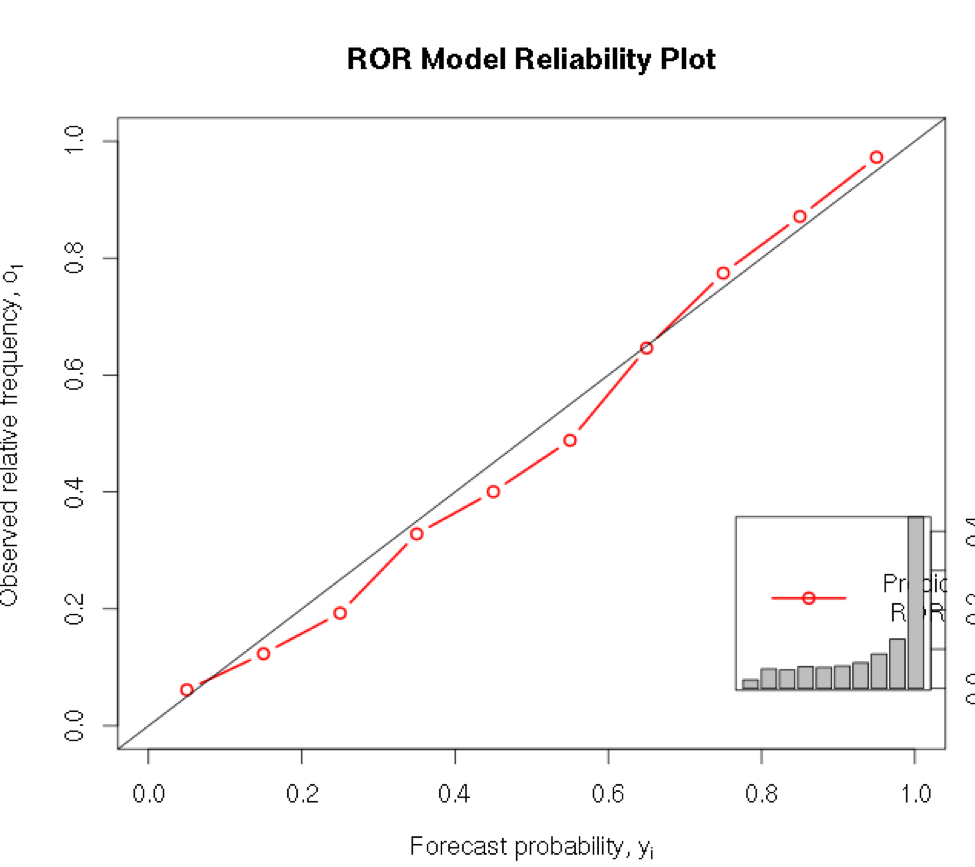
\includegraphics[width=\textwidth]{figures/appd.png}
                  \label{fig:AppD}
                \end{subfigure}
      \end{subfigure}
      \caption{Random Forest Model}
\end{figure}
\newpage

\begin{figure}[h]
  \centering
    \begin{subfigure}[p!]{\textwidth}
    \caption{ROR Modeling using GLM}
        \begin{subfigure}[p1]{0.49\textwidth}
            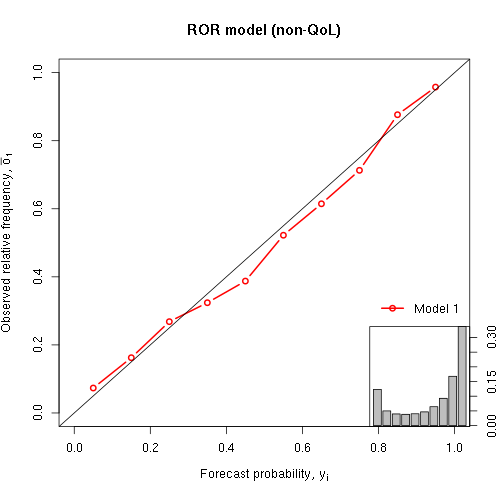
\includegraphics[width=\textwidth]{figures/glmplots/ror_fc.png}
        \end{subfigure}
        ~
        \begin{subfigure}[p1]{0.49\textwidth}
            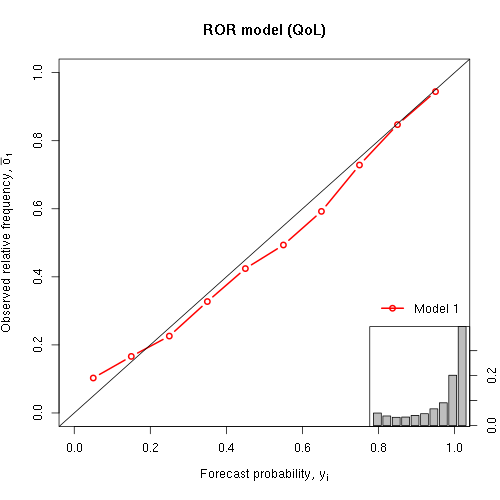
\includegraphics[width=\textwidth]{figures/glmplots/rorq_fc.png}
        \end{subfigure}
    \end{subfigure}


    \begin{subfigure}[p!]{\textwidth}
    \caption{Plea Rates Modeled using GLM}
        \begin{subfigure}[p1]{0.49\textwidth}
            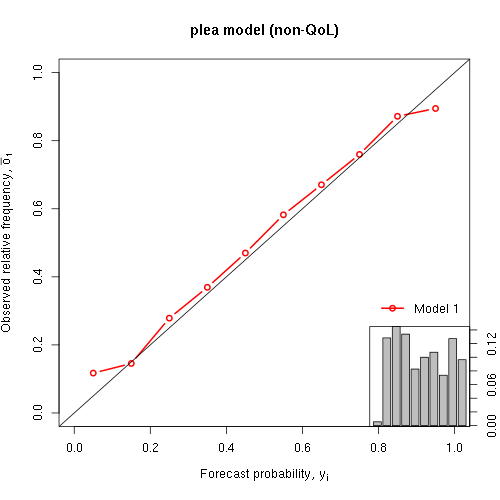
\includegraphics[width=\textwidth]{figures/glmplots/plea_fc.png}

        \end{subfigure}
        ~
        \begin{subfigure}[p1]{0.49\textwidth}
            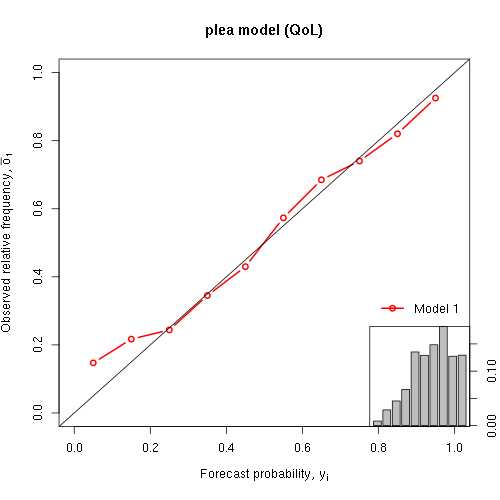
\includegraphics[width=\textwidth]{figures/glmplots/pleaq_fc.png}

        \end{subfigure}
    \end{subfigure}

\end{figure}

\subsection{Validating GLM}
With a half and half test/train split,
the ROR model had acceptable performance,
while the plea model's performance was rather unremarkable.
Though their accuracy rates are not abysmal,
it is important to keep in mind that
both outcomes being predicted have relatively high frequency in the data
(ROR rate is close to 65 percent and plea rate is around 50 percent).




\newpage
\bibliography{../../../references.bib}

\end{document}
